\documentclass[tikz,border=5mm]{standalone}
\usetikzlibrary{decorations.pathmorphing}

\begin{document}
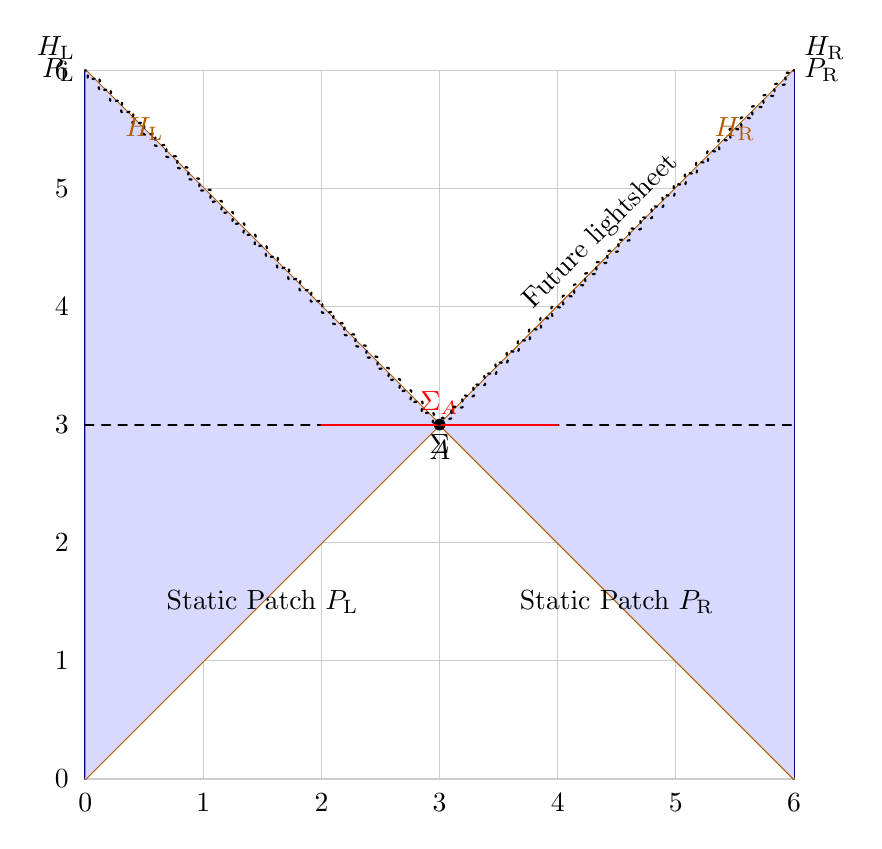
\begin{tikzpicture}[scale=1.5, line cap=round, line join=round]
    % Coordinate system
    \draw[black!20, thin] (0,0) grid (6,6);
    \foreach \x in {0,1,...,6} \node at (\x,-0.2) {\x};
    \foreach \y in {0,1,...,6} \node at (-0.2,\y) {\y};
    
    % Antipodal trajectories (observers)
    \draw[thick, blue!50!black] (0,0) -- (0,6) node[left,black] {$P_{\rm L}$};
    \draw[thick, blue!50!black] (6,0) -- (6,6) node[right,black] {$P_{\rm R}$};
    
    % Cosmological horizons
    \draw[thick, orange!70!black] (0,0) -- (6,6) node[above right,black] {$H_{\rm R}$};
    \draw[thick, orange!70!black] (6,0) -- (0,6) node[above left,black] {$H_{\rm L}$};
    
    % Static patches (blue regions)
    \fill[blue!15] (0,0) -- (0,6) -- (3,3) -- cycle;
    \fill[blue!15] (6,0) -- (6,6) -- (3,3) -- cycle;
    
    % Global spacelike slice (dashed)
    \draw[dashed, thick] (0,3) -- (6,3) node[midway,below] {$\Sigma$};
    
    % Sphere A and its lightsheet
    \node[circle,fill=black,inner sep=1.5pt,label=below:$A$] at (3,3) {};
    \draw[red, thick] (2,3) -- (4,3) node[midway,above] {$\Sigma_A$};
    
    % Future lightsheet (dotted)
    \draw[dotted, thick, decorate,
          decoration={snake,segment length=2mm,amplitude=0.5mm}]
        (3,3) -- (6,6) node[midway,above,sloped] {Future lightsheet};
    \draw[dotted, thick, decorate,
          decoration={snake,segment length=2mm,amplitude=0.5mm}]
        (3,3) -- (0,6);
    
    % Labels
    \node at (1.5,1.5) {Static Patch $P_{\rm L}$};
    \node at (4.5,1.5) {Static Patch $P_{\rm R}$};
    \node[orange!70!black] at (0.5,5.5) {$H_{\rm L}$};
    \node[orange!70!black] at (5.5,5.5) {$H_{\rm R}$};
\end{tikzpicture}
\end{document}